\documentclass[mathserif, aspectratio=169]{beamer}
\usetheme{odenpecos}
\setbeamertemplate{itemize/enumerate body begin}{\fontsize{8.8}{9}\selectfont}
\setbeamertemplate{itemize/enumerate subbody begin}{\fontsize{7.5}{8}\selectfont}
\setbeamertemplate{itemize/enumerate subsubbody begin}{\fontsize{7.5}{8}\selectfont}

% default search path for figures
\graphicspath{{./shared_figures/}{./figures/}}

\newcommand{\zapspace}{\topsep=0pt\partopsep=0pt\itemsep=0pt\parskip=0pt}

\usepackage{multicol}
\usepackage{pict2e}
\usepackage{esdiff}
\usepackage{multimedia}
\usepackage{verbatim}
\usepackage{mhchem}

\usepackage[percent]{overpic}
\usepackage[absolute,overlay]{textpos}

\newcommand{\overbar}[1]{\mkern 1.5mu\overline{\mkern-1.5mu#1\mkern-1.5mu}\mkern 1.5mu}
\newcommand{\pp}[2]{\frac{\partial #1}{\partial #2}}
\newcommand{\dd}[2]{\frac{d #1}{d #2}}
\newcommand{\DD}[2]{\frac{D #1}{D #2}}
\newcommand{\mm}{\mathbf{minmod}}
\def\etal{{\it et al~}}
\newcommand{\be}{\begin{eqnarray}}
\newcommand{\ee}{\end{eqnarray}}
\newcommand{\mbb}[1]{\mathbb{#1}} % math blackboard bold
\newcommand{\mcal}[1]{\mathcal{#1}} % math blackboard bold
\newcommand{\mbf}[1]{\mathbf{#1}} % math bold face (for vectors)
\newcommand{\sbf}[1]{\boldsymbol{#1}} % bold face for symbols
\newcommand{\jump}[1]{\llbracket #1 \rrbracket} % jump operator
\newcommand{\avg}[1]{\langle #1 \rangle} % average operator
\newcommand{\rarrow}{\rightarrow}
\newcommand{\Rarrow}{\Rightarrow}
\newcommand{\LRarrow}{\Leftrightarrow}
\newcommand{\vvvert}{|\kern-1pt|\kern-1pt|}
\newcommand{\enorm}[1]{\vvvert #1 \vvvert}
\newcommand{\nutil}{\tilde{\nu}}
\newcommand{\Var}{\mathrm{Var}}
\newcommand{\Cov}{\mathrm{Cov}}


\definecolor{MyDarkGreen}{rgb}{0,0.45,0.08}
\newcommand{\myred}[1]{{\color{red} #1}}
\newcommand{\myblue}[1]{{\color{blue} #1}}
\newcommand{\mygreen}[1]{{\color{MyDarkGreen} #1}}

\newcommand{\sa}{\nu_{\mathrm{sa}}}
\newcommand{\tep}{\tilde{\epsilon}}
\newcommand{\Ssd}{\mathcal{S}} % source term due to slow derivative
\newcommand{\ud}{\,\mathrm{d}}

\newcommand{\Mach}[1]{\ensuremath{\mbox{Ma}_{#1}}}
\newcommand{\Reynolds}{\ensuremath{\mathit{Re}}}
\newcommand{\DensityRat}{\ensuremath{\mathit{DR}}}
\newcommand{\BlowRat}{\ensuremath{\mbox{BR}}}
\newcommand{\VelRat}{\ensuremath{\mathit{VR}}}
\newcommand{\Tau}{\ensuremath{\mathrm{T}}}

\newcommand{\wall}     {\ensuremath{\mathrm{w}}}   % wall subindex
\newcommand{\awall}    {\ensuremath{\mathrm{aw}}}  % adiabatic wall subindex

\newcommand{\commentout}[1]{}

\newcommand{\vect}[1]{\boldsymbol{#1}}
\usepackage{mleftright}
\newcommand{\of}[1]{\mleft( #1 \mright)}
\newcommand{\vth}{v_{\textrm{th}}}
\newcommand{\reals}{\mathbb{R}}
\newcommand{\myint}[2]{\int\limits_{#1}^{#2}}

\DeclareMathOperator{\variance}{Var}

\begin{document}
% disable nav
\setbeamertemplate{navigation symbols}{}

%===============================================================================
\begin{frame}
\begin{center}
{Solving the Boltzmann equation for electron kinetics using Petrov-Galerkin approach \\ 
{\tiny Milinda Fernando, Daniil Bochkov, Todd Oliver, George Biros}}
\end{center}
%
\scalebox{0.7}{
\begin{columns}[T]
\begin{column}{.71\linewidth}
\begin{itemize}
\item \textbf{Importance:} 
%Electron density function $f_e = f_e(\vect{x}, \vect{v}, t)$ defines transport and kinetic properties
Distribution function of electrons defines transport and kinetic properties
\\
$\rightarrow$ Need to couple plasma model with electron kinetics (Y3)
\item Evolution of $f_e = f_e(\vect{x}, \vect{v}, t)$ obeys the \textbf{Boltzmann equation}
\begin{align*}
\partial_t f_e + \vect{v}\cdot \nabla_{\vect{x}} f_e  + \vect{L} \cdot \nabla_{\vect{v }}f_e = \sum_{a} C_a(f_e)
\end{align*}
where, for example, in case of $a=$ elastic collisions
\begin{align*}
C_a(f_e) &= n_0\int_{S^2} v \underbrace{\sigma_a(v,\omega)}_{\tiny\text{\tiny scat. cross sec.}} 
\left( f_e(v^\prime) - f_e(v) \right) \ud \omega 
\end{align*}
\item \textbf{Main challenge}: 6+1 dimensions
\item \textbf{Idea}: FEM in $\vect{x}$, spectral in $\vect{v}$
\item \textbf{Currently (Y1)}: spatially homogeneous case $f = f(\vect{v}, t)$ 
\begin{align*}
\partial_t f =  \sum_{a} C_a(f_e)
\end{align*}
to investigate efficient velocity-space discretizations
\end{itemize}
\end{column}
\begin{column}{.71\linewidth}
\begin{itemize}
\item \textbf{Approach:} Petrov-Galerkin
\begin{itemize}
\item Nearly isotropic and symmetric $f$ $\rightarrow$ employ spherical harmonics
\item Solution as a perturbed Maxwellian $M\of{v} = n_e \left( \frac{m}{2 \pi kT }\right)^{\frac32} e^{-\frac{mv^2}{2kT}}$: 
\begin{align*}
f\of{\vect{v}}
= M\of{v} \sum_{k,l,m} h_{k,l,m} \of{t} \Phi_k\of{v} \underbrace{Y_{lm}\of{v_\theta, v_\phi}}_{\tiny\text{sph. harm.}}
\quad \rightarrow \quad \text{ODEs for } h_{k,l,m} \of{t}
%M\of{v} = \frac{n}{\left( \vth \sqrt{\pi} \right)^3} e^{-\left(\frac{v}{\vth}\right)^2}
%M\of{v} = n_e \left( \frac{m}{2 \pi kT }\right)^{\frac32} e^{-\frac{mv^2}{2kT}}
%, \quad
%\vth = \sqrt{\frac{2kT}{m}}
\end{align*}
%\begin{align*}
%\rightarrow \quad \sum_{k,l,m} M_{p,q,s}^{k,l,m} \partial_t h_{k,l,m}\of{t} = \sum_{k,l,m}  L_{p,q,s}^{k,l,m} h_{k,l,m}\of{t}
%\end{align*}
\end{itemize}
\end{itemize}
\begin{columns}[T]
\begin{column}{.5\linewidth}
%\begin{itemize}
%\item 
\begin{itemize}
\item[] \textbf{Results:}
\item Invetigating choice of $\Phi_k(v)$:
\begin{itemize}
\item Tested Laguerre, Maxwell, Chebyshev, Linear polys using Bolsig+ data
\end{itemize}
\item Solver implementation:
\begin{itemize}
\item Python
\item Tenzorized 5D integrations: \\0.0093s vs 5.2256s loop-based
\item Arbitrary choice of $\Phi_k(v)$
\item Reactions implemented:
Elastic, Excitation, Ionization
\item Testing and verification are underway
\end{itemize}
\end{itemize}
%\end{itemize}
\end{column}
\begin{column}{.5\linewidth}
\begin{center}
\vspace{-0.2in}
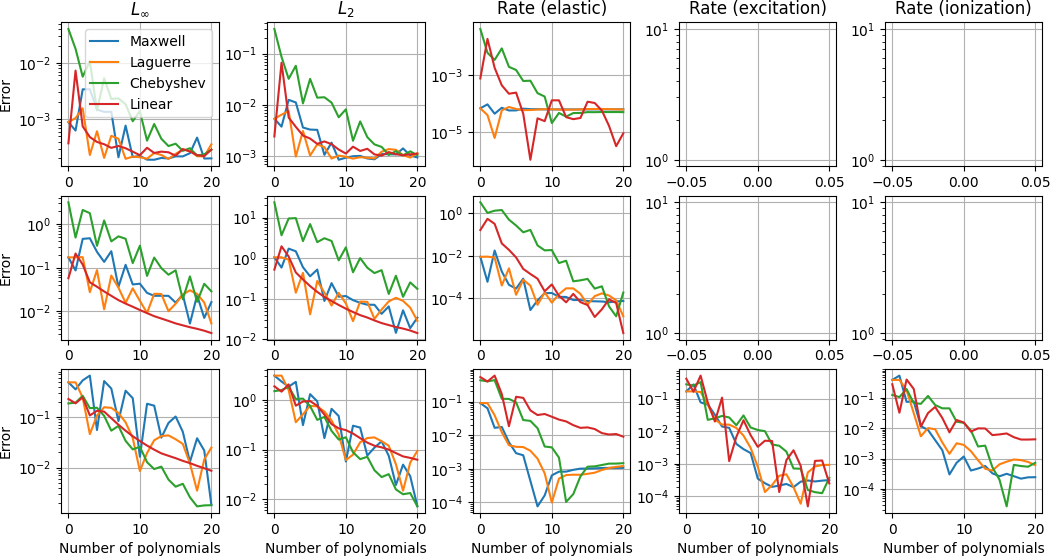
\includegraphics[width=.99\textwidth]{figures/bolsig_convergence.png}
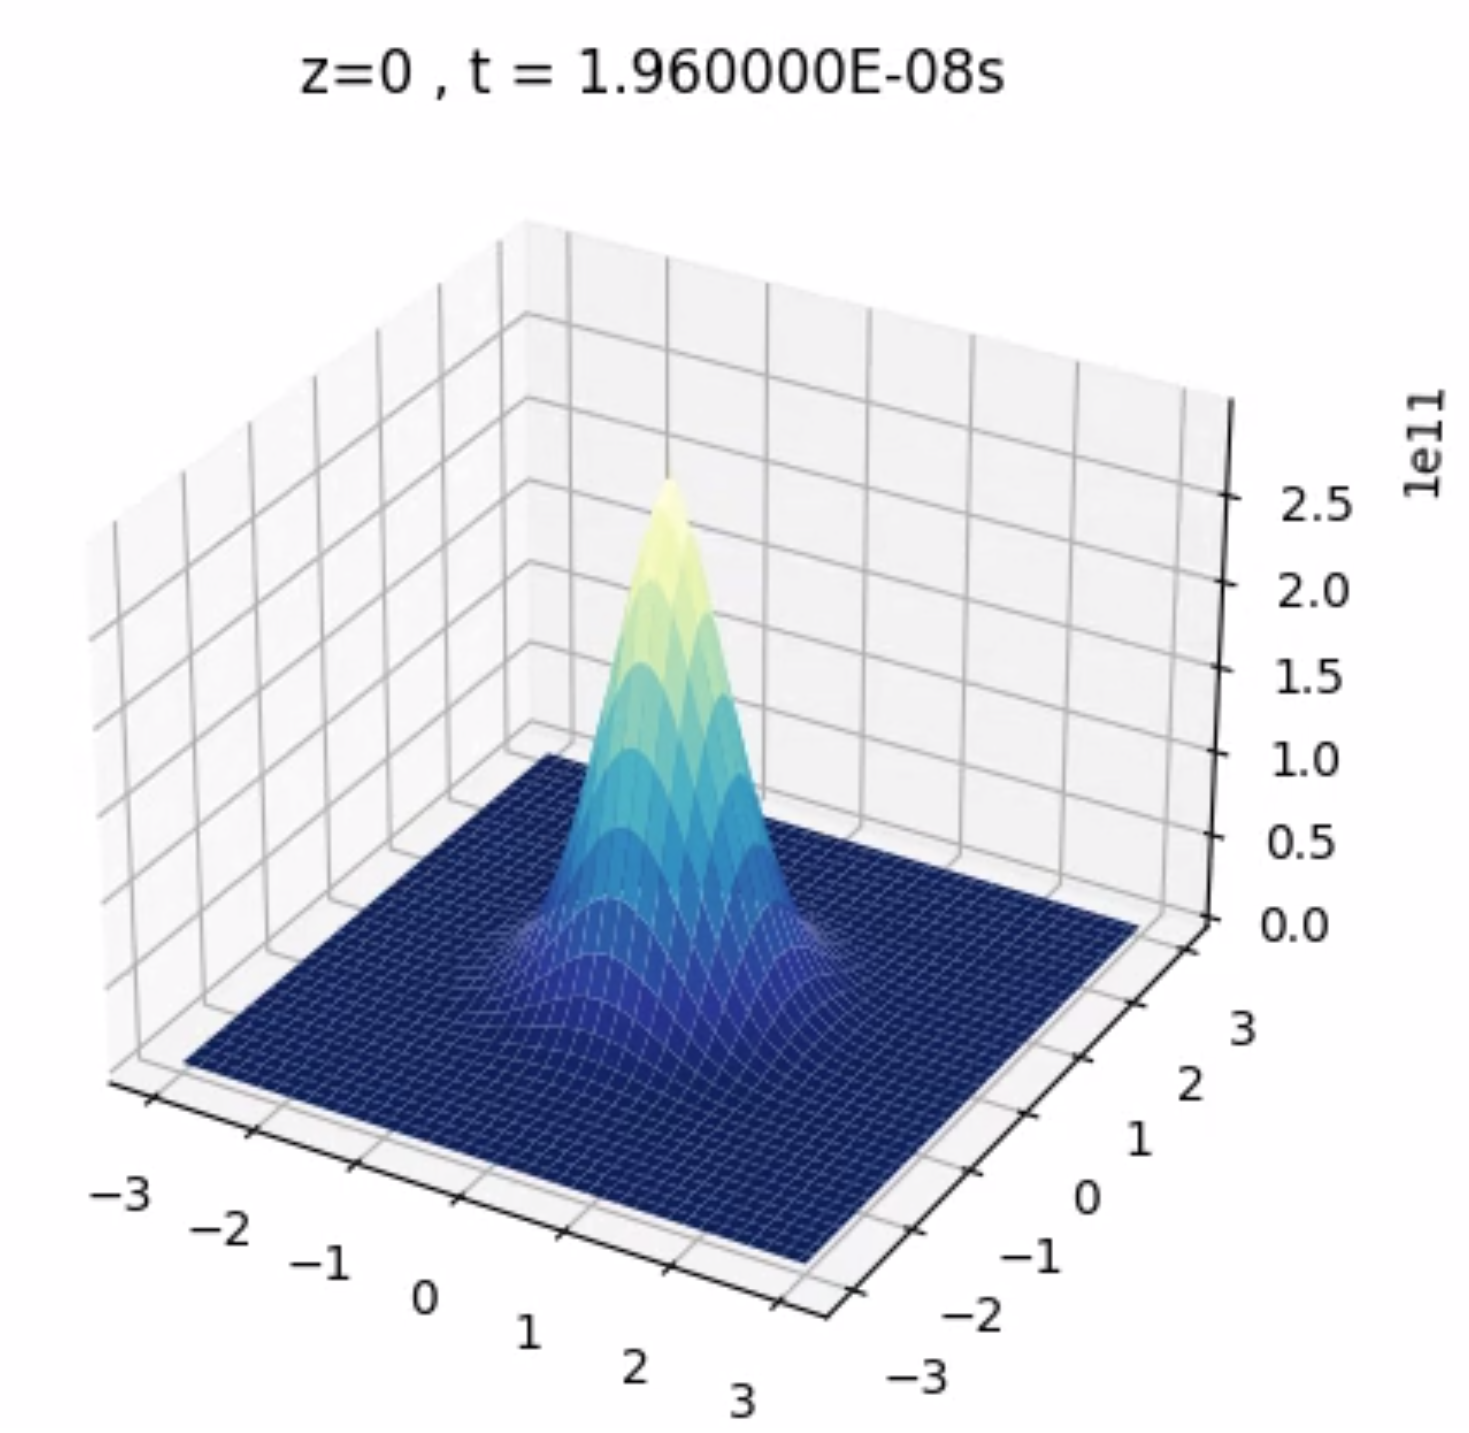
\includegraphics[width=.5\textwidth]{figures/code.png}
\end{center}
\end{column}
\end{columns}
\end{column}
\end{columns}
}
%
\end{frame}
\end{document}

